
\chapter{�berblick und Struktur von TCP/IP}

TCP/IP ist bez�glich der Funktionen ebenfalls in Schichten aufgeteilt,
auch wenn die Schnittstellen zwischen den Schichten (im Gegensatz
zum ISO/OSI Modell) nicht definiert sind. Es wird oft eine Abbildung
der Schichten vom TCP/IP Stack zum OSI Modell vorgenommen. Auf der
untersten Ebene gibt es wieder die Bit�bertragungsschicht, dar�ber
die Sicherungsschicht, dar�ber die Vermittlungsschicht und zum Schluss
die Transportschicht. Dar�ber hinaus gibt es nur noch eine Anwendungsschicht
und die eigentlichen Anwendungen.
\begin{itemize}
\item D.h. der TCP/IP Protokollstack l�sst sich in diesem Sinne als ein
Schichtenmodell von 4 Schichten beschreiben, die jeweils 4 Schichten
im ISO/OSI Referenzmodell zugeordnet werden k�nnen:
\item Als unterste Schicht dient die Verbindungsschicht (engl. auch network
interface layer genannt), die die Bit�bertragungsschicht \emph{und}
die Sicherungsschicht des ISO/OSI Modells umfasst.
\item Darauf baut die Internetschicht (engl. internet layer) auf, die der
Vermittlungsschicht im ISO/OSI Modell entspricht. In dieser Schicht
gibt es in TCP/IP die Protokolle Internet Protocol (IP), Internet
Control Message Protocol (ICMP), das Address Resolution Protocol (ARP)
und das Reverse Address Resolution Protocol (RARP).
\item Die n�chste Schicht ist die Transportschicht (engl. transport layer),
die wiederum direkt auf die Transportschicht im ISO/OSI Modell abgebildet
werden kann. Im TCP/IP Modell gibt es zwei verschiedene Transportprotokolle:
Transport Control Protocol (TCP) und User Datagram Protokoll (UDP).
\item Als n�chste Schicht folgt im TCP/IP Modell direkt die Anwendungsschicht,
die hiermit auch die Funktionen der Sitzungsschicht und der Darstellungsschicht
beinhalten muss. F�r diese beiden Schichten des ISO/OSI Modells gibt
es in TCP/IP kein Gegenst�ck.
\end{itemize}
Die Abbildung \vref{fig:tcpip_layers} stellt die Schichten und die
Querverbindungen dar. Es ist daraus auch zu erkennen, dass das TCP/IP
Modell eigentlich kein striktes Schichtenmodell implementiert.

%
\begin{figure}
\centering

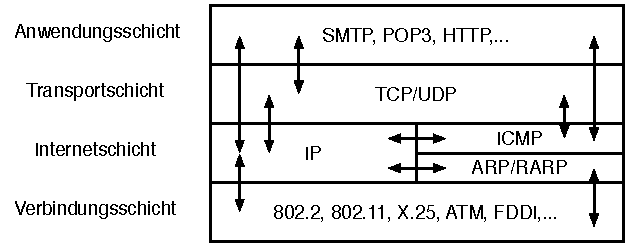
\includegraphics[bb=0bp 0bp 138mm 42mm,clip]{tcpip_overview/tcpip_layers}

\caption{\label{fig:tcpip_layers}TCP/IP Schichtenmodell}

\end{figure}


Man sieht, dass in der Verbindungsschicht nicht nur IP (der eigentliche
Kern von TCP/IP) angesiedelt ist, sondern noch weitere Protokolle,
die nicht direkt zu IP geh�ren, jedoch ein integraler Bestandteil
dieser Schicht sind. Dies ist einerseits ICMP, das haupts�chlich zur
Benachrichtigung von Fehlern in der Internetschicht dient und die
Protokolle ARP und RARP, die zur Umsetzung von IP Adressen in Hardwareadressen
(wie z.B. Ethernet-MAC-Adressen) bzw. umgekehrt dienen.

Der Hauptzweck der Internetschicht liegt in der globalen Adressierung
der Hosts und der �bertragung der Pakete zwischen den Hosts.

In der Transportschicht gibt es zwei Protokolle, n�mlich das verbindungsorientierte,
zuverl�ssige TCP und das verbindungslose, unzuverl�ssige UDP.

Die Anwendungsschicht ist in den eigentlichen TCP/IP Standards nicht
beschrieben und muss, wie schon erw�hnt, ebenfalls die Funktionen
der Sitzungsschicht und der Darstellungsschicht �bernehmen. D.h. obwohl
der TCP/IP Protokollstack vom Prinzip her ebenfalls eine Anwendungsschicht
vorsieht, es jedoch keinen Standard gibt, ist jede Anwendung aus diesem
Grund daf�r selbst zust�ndig die ben�tigten Funktionen der Sitzungsschicht,
der Darstellungsschicht und der Anwendungsschicht zu implementieren.

Die Protokolle IP, TCP, UDP, ICMP und ARP werden in weiterer Folge
noch genauer beschrieben.
